\documentclass[tikz,border=2pt]{standalone}
\usepackage{amsmath,amssymb}
\usepackage{tikz}

\begin{document}
% E is an open blob (dashed edge). Every point of E and every point of its edge is adherent:
% each ball around it meets E. The closure adds the edge (solid curve). A point further away
% has a ball that misses E, so it is not adherent.
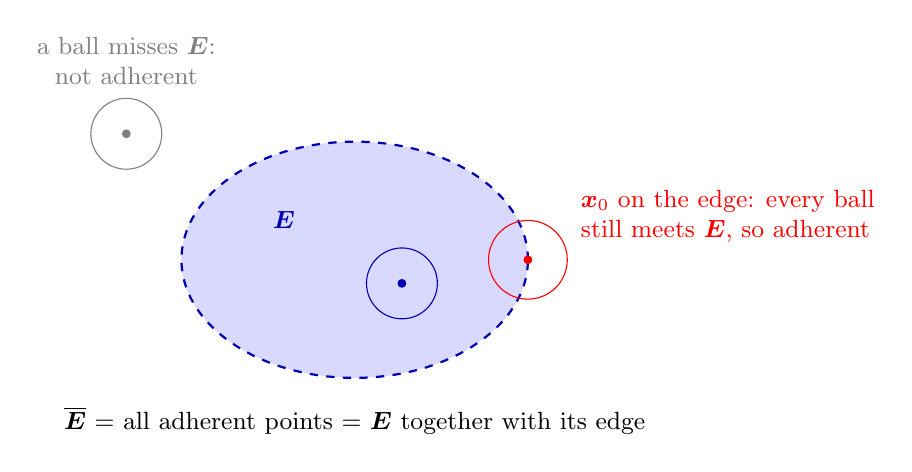
\begin{tikzpicture}[every node/.style={font=\small}]
	\fill[blue!15] (0,0) ellipse (2.2 and 1.5);
	\draw[blue!70!black, thick, dashed] (0,0) ellipse (2.2 and 1.5);
	\node[blue!70!black] at (-0.9,0.5) {$\boldsymbol{E}$};
	% interior adherent point
	\fill[blue!70!black] (0.6,-0.3) circle (1.6pt);
	\draw[blue!70!black] (0.6,-0.3) circle (0.45);
	% boundary adherent point (on the edge, not in E)
	\fill[red] (2.2,0) circle (1.6pt);
	\draw[red] (2.2,0) circle (0.5);
	\node[red, anchor=west, align=left] at (2.75,0.55) {$\boldsymbol{x}_0$ on the edge: every ball\\ still meets $\boldsymbol{E}$, so adherent};
	% non-adherent point
	\fill[gray] (-2.9,1.6) circle (1.6pt);
	\draw[gray] (-2.9,1.6) circle (0.45);
	\node[gray, anchor=south, align=center] at (-2.9,2.1) {a ball misses $\boldsymbol{E}$:\\ not adherent};
	\node[anchor=north, align=center] at (0,-1.75) {$\overline{\boldsymbol{E}}$ = all adherent points = $\boldsymbol{E}$ together with its edge};
\end{tikzpicture}
\end{document}
